\documentclass[a4paper,11pt]{article}

\usepackage{amsmath,amssymb,graphicx}
\usepackage[margin=2cm]{geometry}
\linespread{1.35}
\setlength{\parskip}{6pt}
\setlength{\parindent}{0pt}
\usepackage{fancyhdr}
\pagestyle{fancy}

\begin{document}

\title{\textsc{This is My First LaTeX Document} \\ \small Lab2 Practice}
\author{\Large{Your Name} \\ \small Student ID}
\date{\today}
\maketitle

\section{Borrowed Words}

\textbf{Quotations} are often used in a document, either to add \textit{weight} to our arguments by referring to a higher authority or because we find that we cannot improve on the way an idea has been expressed by someone else. Consider the following example, a quotation from \textsc{Bertrand Russell}.

Some mathematicians elevate the spirit of Mathematics to a kind of intellectual aesthetics. It is best voiced by Bertrand Russell in the following lines.

\textit{
The true spirit of delight, the exaltation, the sense of being more than man, which is the touchstone of the highest excellence, is to be found in Mathematics as surely as in poetry. Real life is, to most men, a long second best, a perpetual compromise between the ideal and the possible; but the world of pure reason knows no compromise.}

Yes, to men like Russell, Mathematics is more of an art than science.

\newpage
\section{Making Lists}

\subsection{Bullet Lists}

For \textbf{Bullet Lists} use the \texttt{itemize} command. Try to make the following list.

One should keep the following in mind when using \TeX:
\begin{itemize}
\item \TeX\,  is a typesetting language and not a word processor,
\item \TeX \, is a program and not an application,
\item \TeX \, there is no meaning on comparing \TeX \, to a word processor, since the design purposes are different.
\end{itemize}
Being a program, \TeX \, offers a high degree of flexibility.

\subsection{Numbered Lists}

For numbered lists use \texttt{enumerate}. Make the following list.

The three basic steps in producing a printed document using \LaTeX are as follows:
\begin{enumerate}
\item Prepare a source file with the extension \texttt{.tex}
\item Compile it with \LaTeX to produce a \texttt{dvi} file
\item Print the document using a \texttt{dvi} driver
\end{enumerate}

\subsection{Multilevel Lists}

Multilevel lists are usually combinations of numbered and bulleted lists. Try to create the following list.

There are \textbf{three levels} in the following list:
\begin{enumerate}
\item First item in the \underline{first} level
\item Second item in the first level
\begin{enumerate}
\item[i.] first item in the \underline{second} level
\item[ii.] second item in the second level
\item[iii.] third item in the second level
\begin{itemize}
\item[-] first item in the \underline{third} level
\item[-] second item in the third level
\end{itemize}
\end{enumerate}
\end{enumerate}
That is it; a multilevel list.

\newpage
\section{Truth Table}

I hope you still remember the \textbf{\textit{Truth Tables}} from CELEN086, last Semester!! Try to create the following Truth Table.

\begin{table}[h]
\centering
\begin{tabular}{c|c|c|c}
$p$ & $q$ & $p \vee q$ & $p \wedge q$ \\
\hline
\hline
T & T & T & T \\
T & F & T & F \\
F & T & T & F \\
F & F & F & F\\
\end{tabular}
\caption{The Truth Table for AND, OR gates.}
\end{table}

Can you create this table?
\begin{table}[h]
\centering
\begin{tabular}{l|c c c}
 &  &Year \\
\cline{2-4}
City & 2006 & 2007 & 2008 \\
\hline
London & 45678 & 445768 & 55666\\
Berlin & 34567 & 32456 & 29876\\
Paris & 49876 & 51000 & 51987 \\
Istanbul& 667788 & 668890 & 676869\\
Cairo & 69876 & 65432 & 54300\\
\hline
\end{tabular}
\caption{Some figures about some famous cities}
\end{table}

\subsection{Figures}
In \LaTeX we can include figures and pictures very easily using the\underline{ \texttt{graphicx}} package. Below is a picture of Euler, Swiss mathematician and scientist. The scale is 0.5.
\begin{figure}[h]
\centering
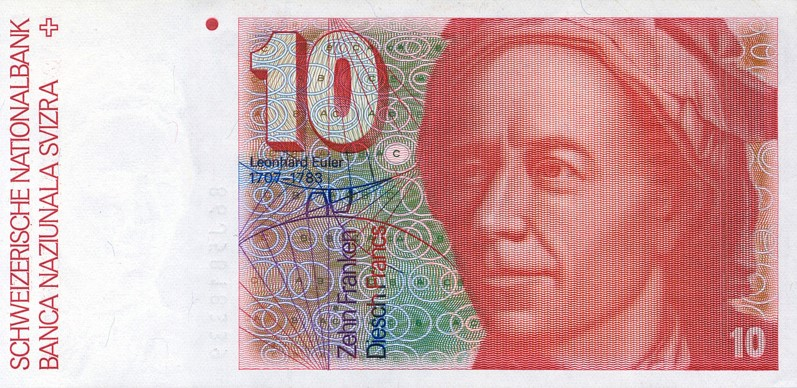
\includegraphics[scale=0.5]{Euler}
\caption{Leonhard Euler(1707-1783)}
\end{figure}


\section{Mathematics}

\subsection{Solving Quadratic Equations}

There is an \textit{exact} method for solving quadratic equations of the form $ax^2+bx+c=0$ where $a, b$ and $c$ are real numbers ($\in \mathbb{R}$). We first compute $\Delta$ (\textit{delta}):
\begin{equation} \Delta = \sqrt{b^2-4ac}. \end{equation}

Now, depending on the \textbf{sign} of $\Delta$ we can determine the quality of the roots:
\begin{equation*}
\Delta 
\begin{cases}
>0 & \quad \textrm{two real roots,} \qquad x_{1,2}=\frac{-b \pm \sqrt{\Delta}}{2a}\\
=0 & \quad \textrm{one real root,} \qquad x_{1,2}=\frac{-b}{2a}\\
<0 & \quad \textrm{NO real roots, complex conjugates} \qquad x_{1,2}=\frac{-b \pm \sqrt{\Delta}\,i}{2a}
\end{cases}
\end{equation*} 
 
\subsection{Derivatives}

The table below shows first and second derivative of some well-known functions.

\begin{table}[h]
\centering
\begin{tabular}{|c|c|c|}
\hline
 $y$ & $y'$ & $y''$\\
\hline
$x^n$ & $nx^{n-1}$ & $n(n-1)x^{n-2}$\\
$\sqrt[3]{x}$ & $\frac{1}{3}x^{-2/3}$ & $\cdots$ \\
$\sin x$ & $\cos x$ & $-\sin x$\\
$\ln x$ & $\frac{1}{x}$ & $\frac{-1}{x^2}$\\
$\frac{1}{x+1}$ & $\frac{-1}{(x+1)^2}$ & $\frac{2}{(x+1)^3}$\\
\hline
\end{tabular}
\end{table}

\subsection{Integration}
Integration is the opposite of differentiation. For a real function $f(x)$ we have the following relationship:

\begin{equation}
\int f(x) dx = F(x)+C,
\end{equation}
where $f(x)=\frac{d}{dx} F(x)$.

Also, an integral represents the area under a curve, that is the area between the curve and the $x-$axis. The following integral gives the area under $f(x)$ from $x=x_1$ to $x=x_2$:
\begin{equation}
A=\int_{x_1}^{x_2} f(x) dx = F(x_2)-F(x_1).
\end{equation}

Area should always be nonnegative: $A \geq 0$.


\end{document}